\documentclass{beamer}
\usepackage[utf8]{inputenc}
\usepackage[spanish]{babel}
\usepackage{graphicx}
\usepackage{booktabs}
\usepackage{ragged2e}
\usepackage{xcolor}
\definecolor{LightGray}{gray}{0.975}
\definecolor{links}{HTML}{2A1B81}
%\usepackage[urlcolor=blue]{hyperref}
\hypersetup{colorlinks,linkcolor=,urlcolor=blue}

\usepackage{tikz}
\usetikzlibrary{arrows,shapes}

\usepackage{algorithm}
\usepackage{algorithmic}

\usepackage{minted}
\usepackage{xcolor}
\definecolor{LightGray}{gray}{0.975}

\usepackage{listings}

%\usetheme{Warsaw}
\usefonttheme{serif} 

\title[ETL]{Database Administration}
\subtitle{Lecture 06: Extraction - Transformation - Load.}
\author{Pentaho Data Integration.}
\date{\today}

\setbeamertemplate{navigation symbols}{}%remove navigation symbols

\defbeamertemplate*{footline}{shadow theme}
{%
  \leavevmode%
  \hbox{\begin{beamercolorbox}[wd=.5\paperwidth,ht=2.5ex,dp=1.125ex,leftskip=.3cm plus1fil,rightskip=.3cm]{author in head/foot}%
    \usebeamerfont{author in head/foot} Database Administration \hfill \insertshorttitle
  \end{beamercolorbox}%
  \begin{beamercolorbox}[wd=.5\paperwidth,ht=2.5ex,dp=1.125ex,leftskip=.3cm,rightskip=.3cm plus1fil]{title in head/foot}%
    \usebeamerfont{title in head/foot} \hfill \insertframenumber\,/\,\inserttotalframenumber%
  \end{beamercolorbox}}%
  \vskip0pt%
}

\AtBeginSection[]
{
     \begin{frame}<beamer>
     \frametitle{Plan}
     \tableofcontents[currentsection]
     \end{frame}
}

\newcommand{\toRight}[1]{
    \begin{FlushRight}
        {\tiny #1}
    \end{FlushRight}
} % Align to right

\begin{document}

\frame{\titlepage}

\begin{frame}{Database Administration: ETL.}
    \centering
    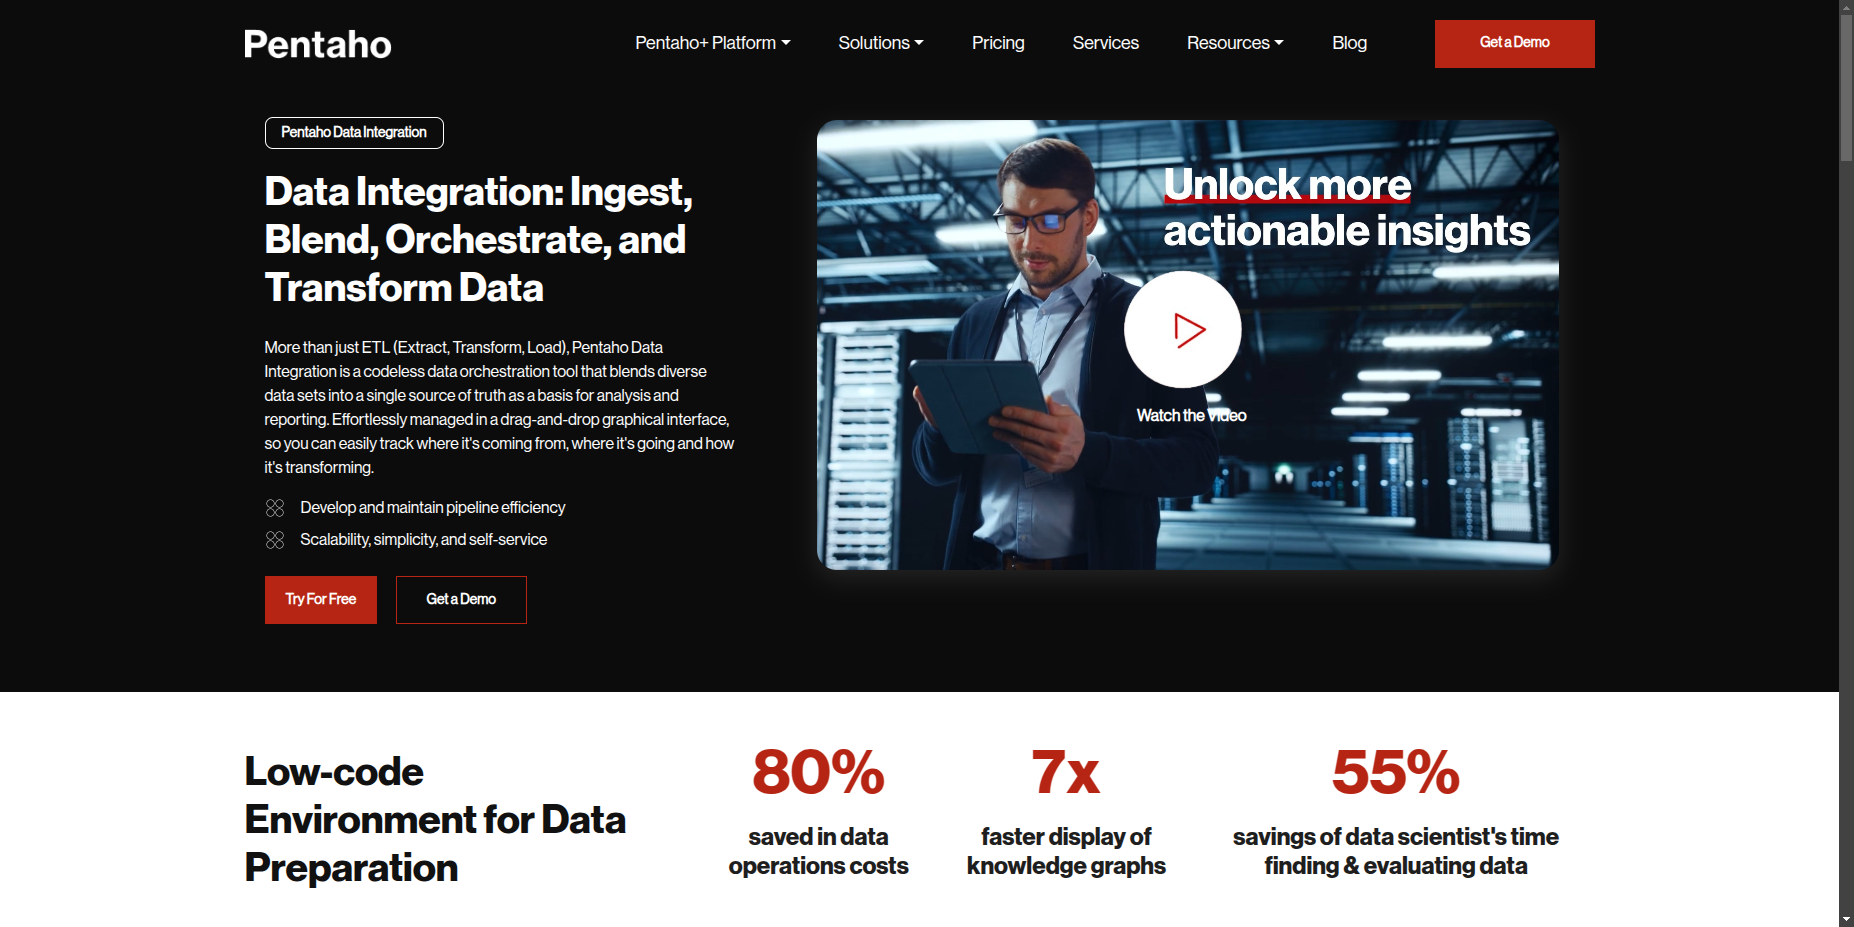
\includegraphics[width=\textwidth]{figures/pdi}\\
    \vspace{2mm}
    {
        \scriptsize
        Content has been extracted from \textit{PDI.} , created by Pentaho Data Integration, 2025.  Visit \url{https://pentaho.com/products/pentaho-data-integration/}.\\
    }
\end{frame}

% Slide: Introduction
\begin{frame}{Pentaho Architecture}
    \centering
    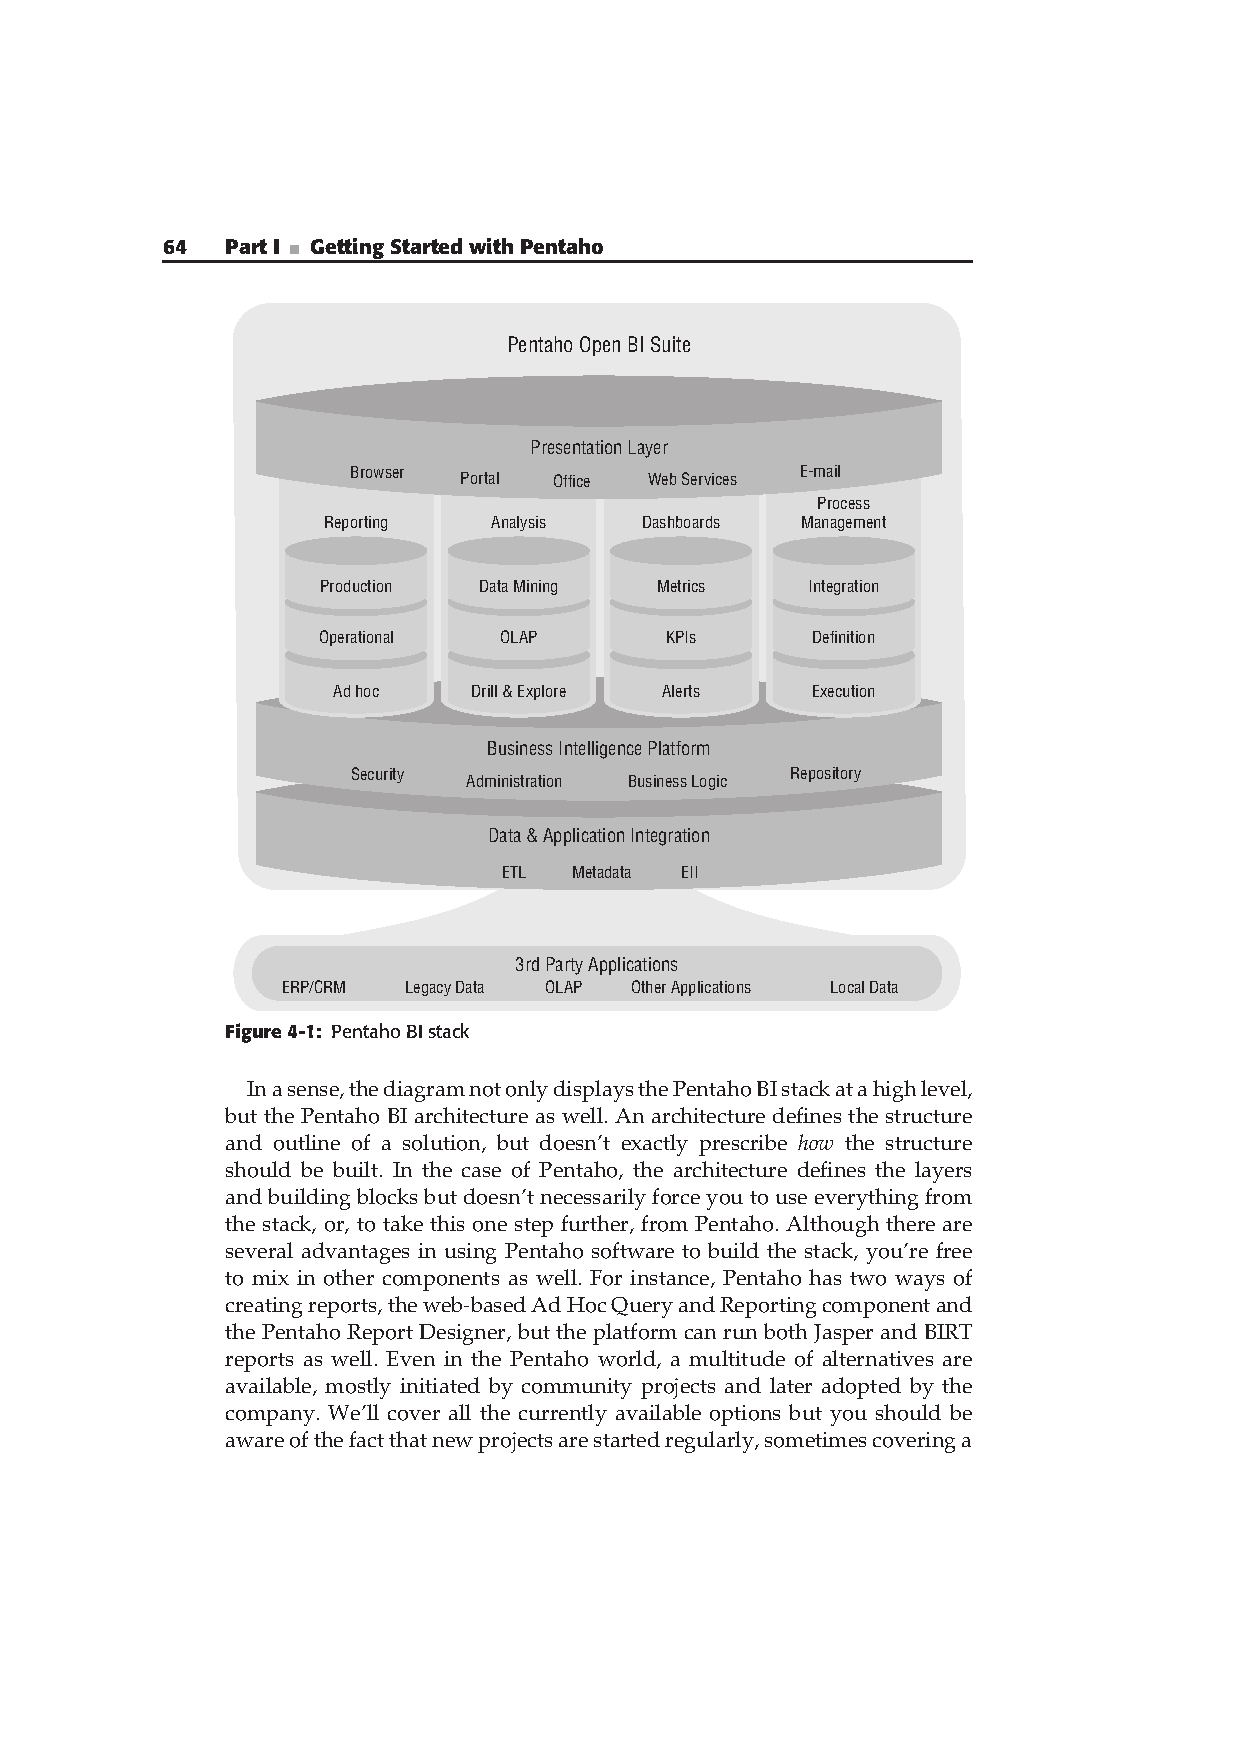
\includegraphics[width=0.95\textwidth, trim={3cm 12.5cm 3cm 5cm}, clip]{figures/pentaho_architecture}  % Add relevant diagram
\end{frame}

\begin{frame}{Introduction}
    \begin{itemize}
        \item Data integration: Combining data from different sources to provide a unified view.
        \item Pentaho Data Integration (PDI) offers tools for ETL (Extract, Transform, Load).
        \item Core PDI components: Transformations, Jobs, and the Data Integration Engine.
    \end{itemize}
\end{frame}

% Slide: Data Integration Activities
\begin{frame}{Data Integration Activities}
    \begin{itemize}
        \item Extraction: Retrieving data from various sources.
        \item Change Data Capture (CDC): Identifying changes in source data.
        \item Data Staging: Intermediate storage for transformation.
        \item Data Validation and Cleansing: Ensuring data quality.
        \item Key Management and Aggregation.
        \item Dimension and Fact Table Loading.
    \end{itemize}
\end{frame}

\begin{frame}{Data Integration Arquitecture}
    \centering
    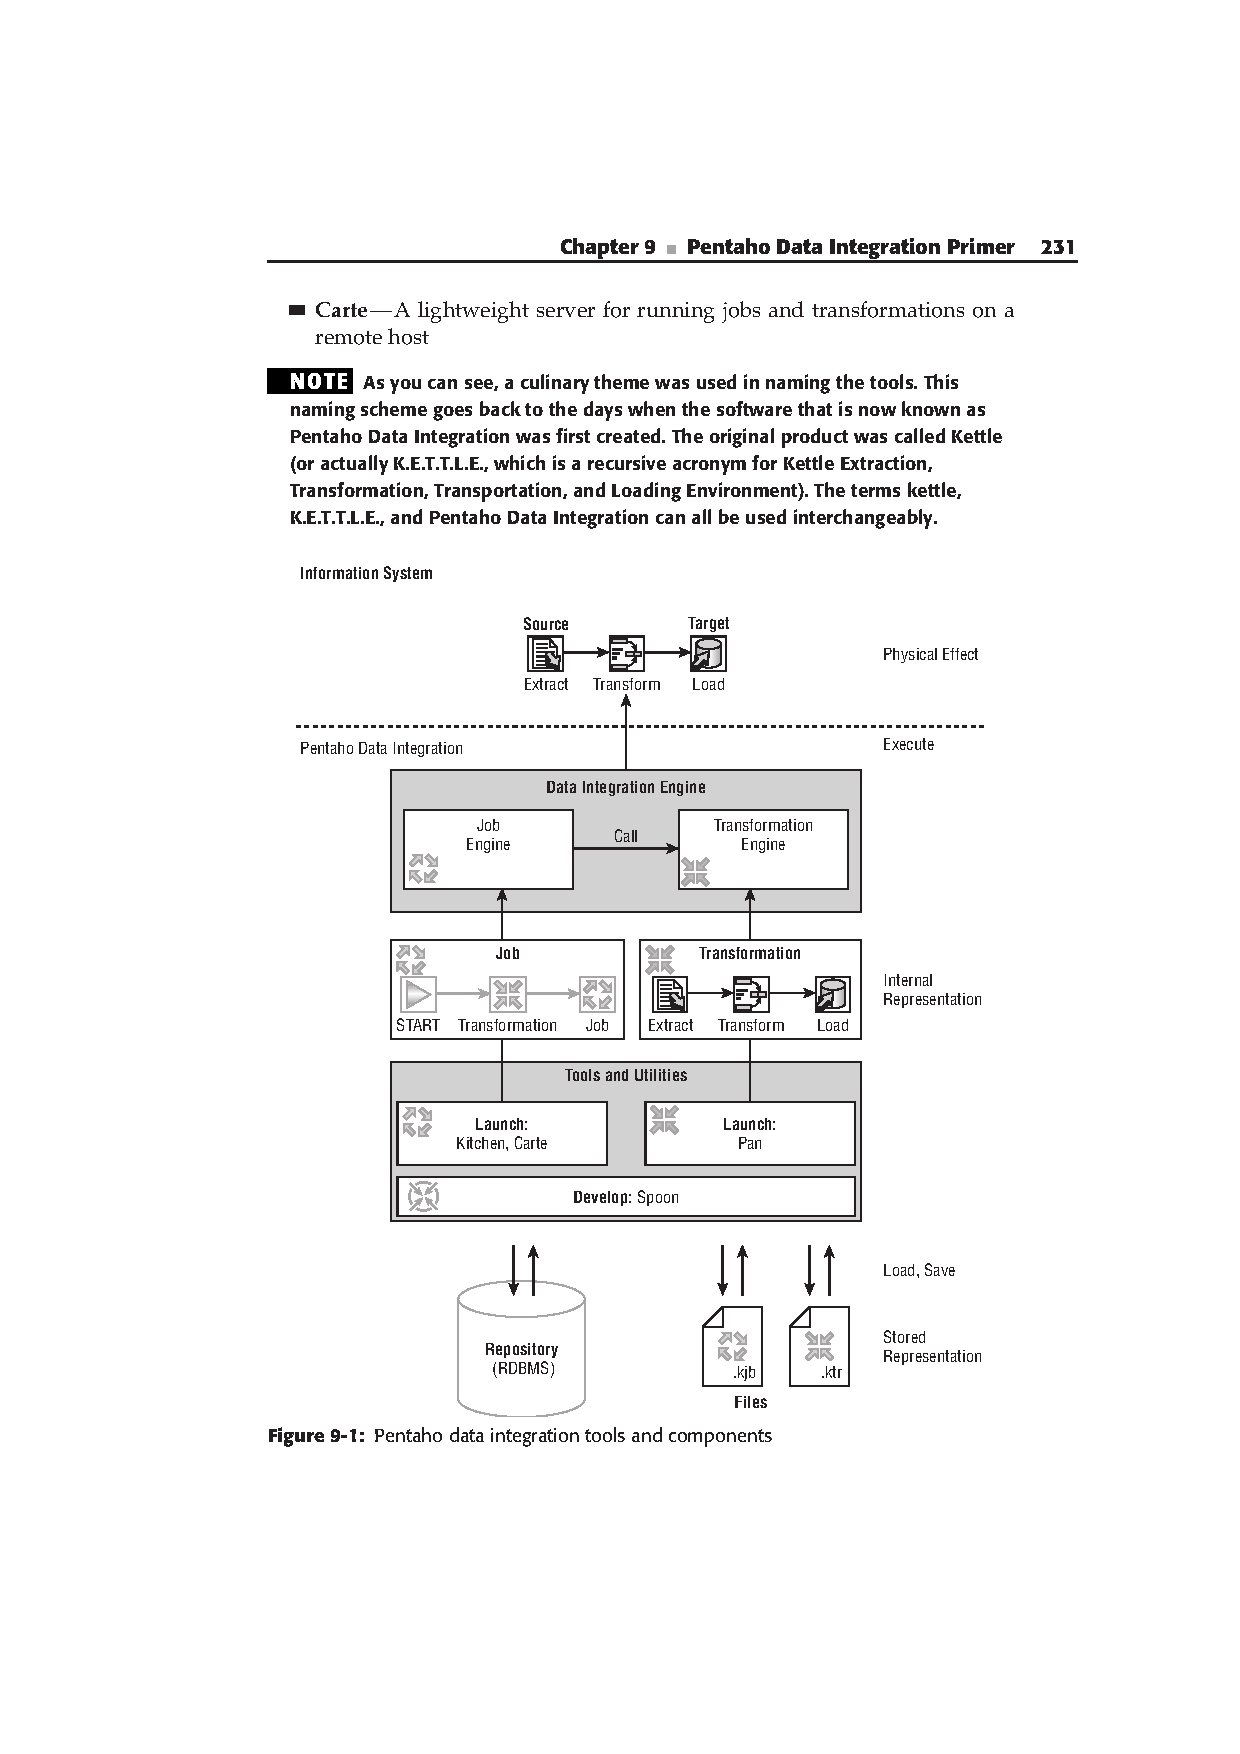
\includegraphics[width=0.7\textwidth, trim={3cm 5.6cm 3cm 10cm}, clip]{figures/pdi_architecture}
\end{frame}

% Slide: Pentaho Data Integration Components
\begin{frame}{Pentaho Data Integration Components}
    \begin{itemize}
        \item \textbf{Spoon}: Graphical IDE for designing transformations and jobs.
        \item \textbf{Kitchen}: Command-line tool for executing jobs.
        \item \textbf{Pan}: Command-line tool for running transformations.
        \item \textbf{Carte}: Remote execution engine.
    \end{itemize}
    \centering
    \vspace{5mm}
    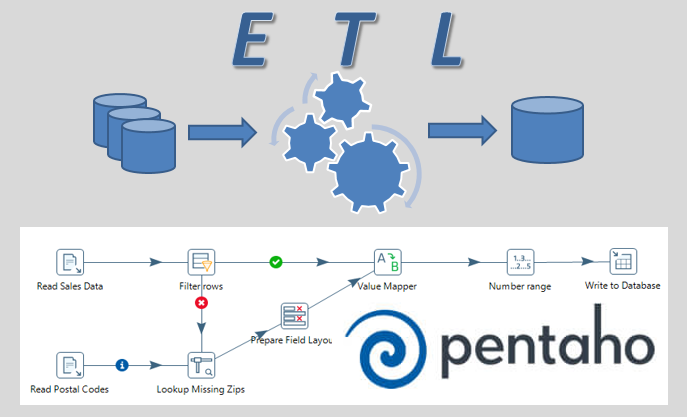
\includegraphics[width=0.6\textwidth]{figures/pdi_components}  % Add relevant diagram
\end{frame}

% Slide: Getting Started with Spoon
\begin{frame}{Getting Started with Spoon}
    \begin{itemize}
        \item Launch Spoon and create a new transformation.
        \item Add steps to extract, transform, and load data.
        \item Connect steps using "hops."
        \item Preview and execute transformations.
    \end{itemize}
    \vspace{2mm}
    \centering
    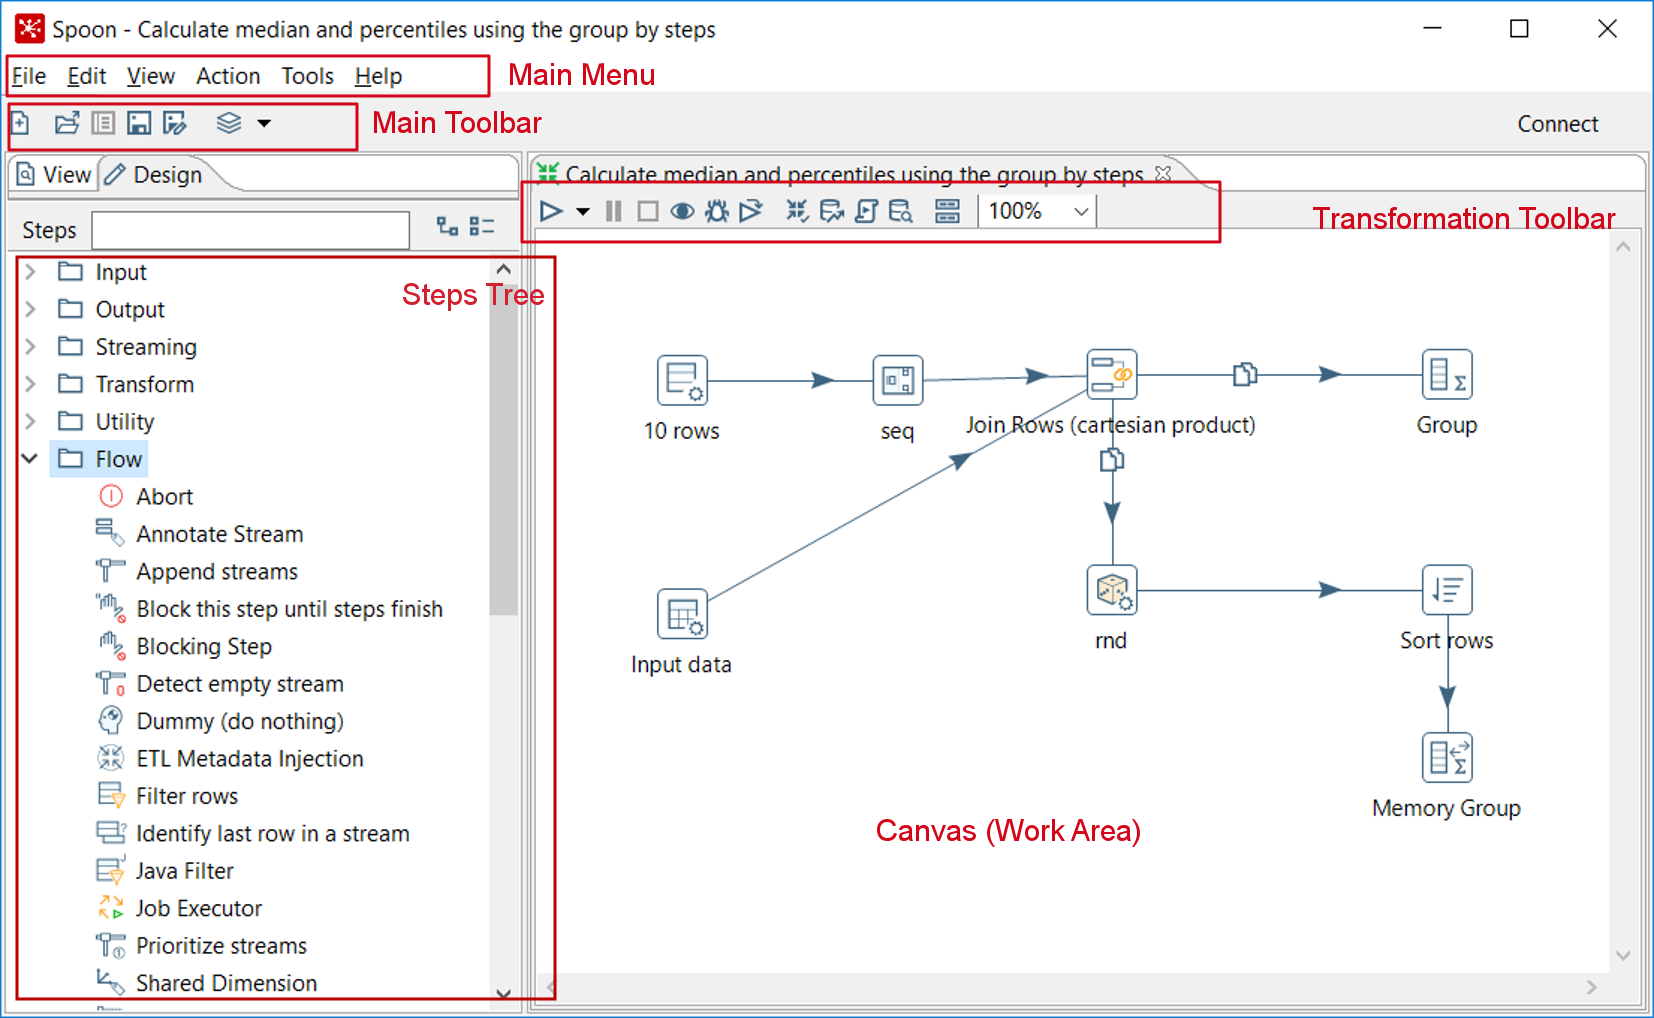
\includegraphics[width=0.8\textwidth]{figures/spoon_ui.png}  % Add Spoon UI screenshot
\end{frame}

% Slide: Summary
\begin{frame}{Summary}
    \begin{itemize}
        \item PDI provides tools for efficient ETL processes.
        \item Transformations process data at the record level.
        \item Jobs orchestrate multiple tasks.
        \item Spoon offers a user-friendly interface for development.
    \end{itemize}
\end{frame}


\begin{frame}{}
    \centering
    \Huge End of Lecture 6.
\end{frame}

\section*{Takeaways}

% Tim Duncan's Top 5 Fundamental Takeaways of the Today's Class
\begin{frame}{TDT5FTOTTC}
    \centering
    
\includegraphics[width=0.75\textwidth]{figures/tim}
\end{frame}

\begin{frame}{Top 5 Fundamental Takeaways}
    \small
    \begin{enumerate}
        \item[5] \pause
        \item[4] \pause
        \item[3] \pause
        \item[2] \pause
        \item[1]
    \end{enumerate}
\end{frame}

\begin{frame}{Database Administration: ETL.}
    \centering
    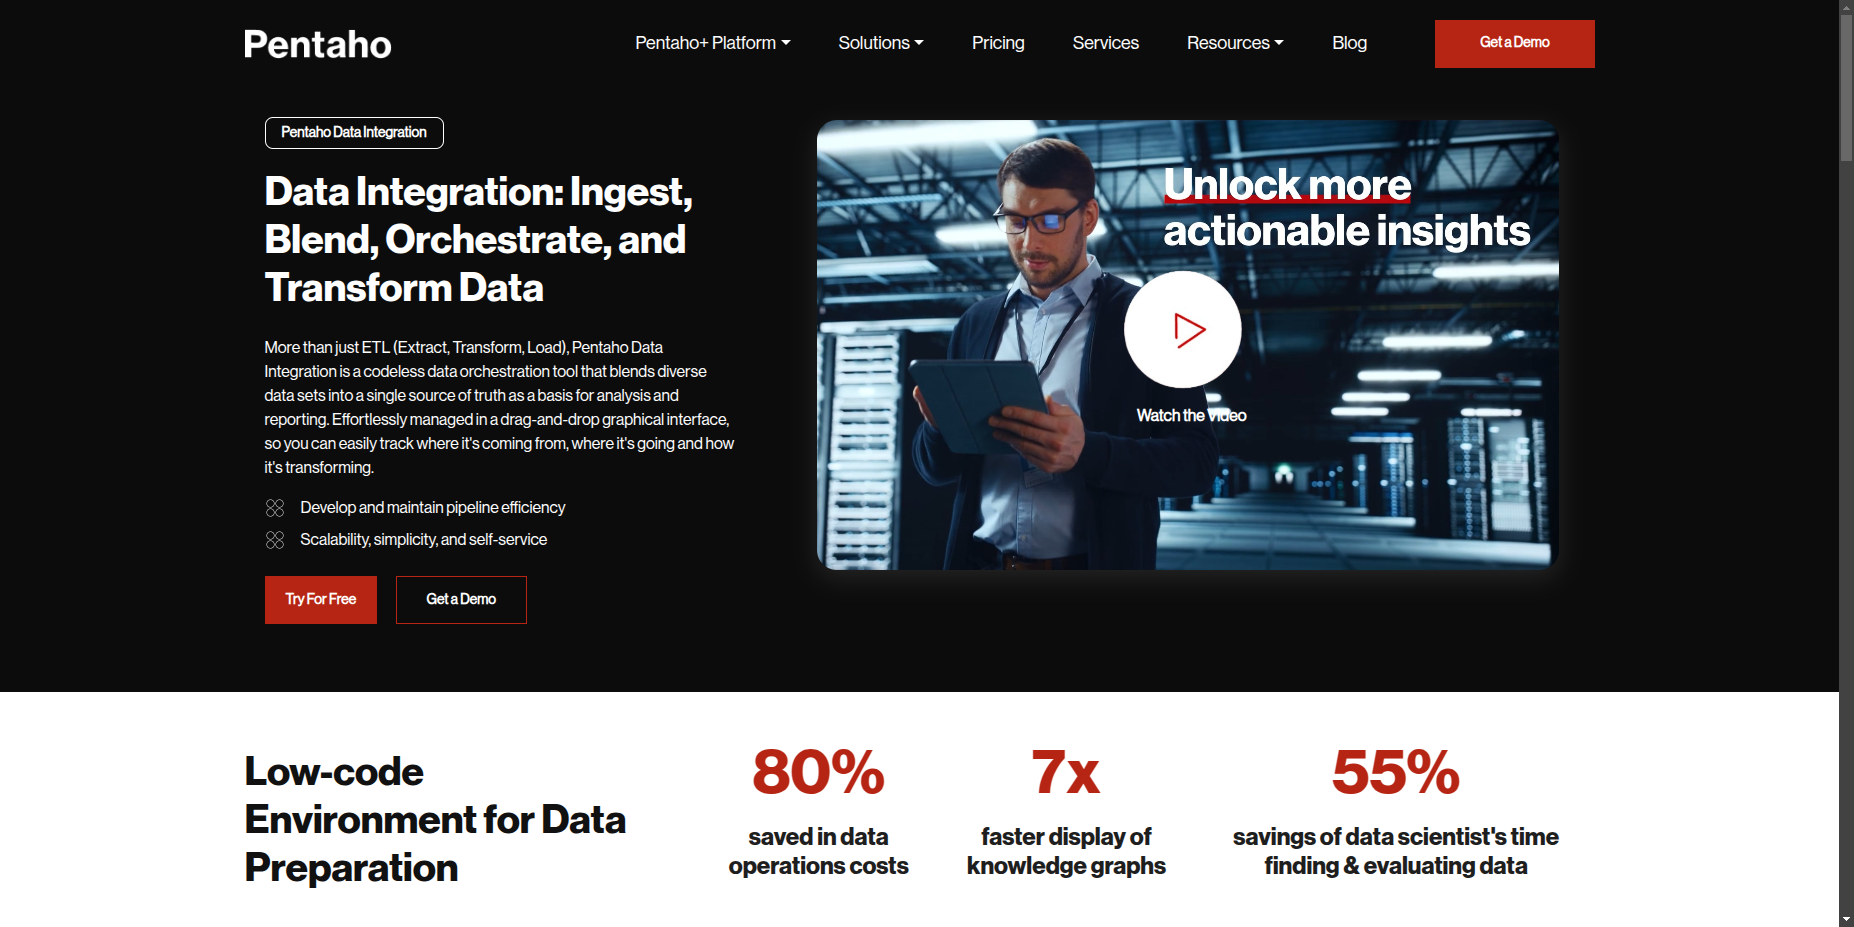
\includegraphics[width=\textwidth]{figures/pdi}\\
    \vspace{2mm}
    {
        \scriptsize
        Content has been extracted from \textit{PDI.} , created by Pentaho Data Integration, 2025.  Visit \url{https://pentaho.com/products/pentaho-data-integration/}.\\
    }
\end{frame}

\end{document}
